\chapter{Autenticazione}

\section{Tipi di Autenticazione}

L'\textbf{autenticazione} è il processo attraverso il quale viene verificata
l'identità di un utente che vuole
accedere ad un computer o ad una una rete. È il sistema che verifica,
effettivamente, che un
individuo è chi sostiene di essere. Stabilisce l'identità di una parte ad un'altra.
Le parti possono essere utenti o computer:

\begin{itemize}
      \item \textbf{computer-computer} (stampa in rete, delega,…)
      \item \textbf{utente-utente} (protocolli di sicurezza, …)
      \item \textbf{computer-utente} (autenticare un server web,…)
      \item \textbf{utente-computer} (per accedere a un sistema…)
\end{itemize}

In realtà sono spesso richieste varie combinazioni di queste.
L'autenticazione è una proprietà primaria, viene richiesta da un corretto
controllo d'accesso.
Garantire l'autenticazione significa fare in modo che un sistema sia in grado di
associare con
certezza un'identità ad una persona.\\

Esistono vari tipi di autenticazione:

\begin{itemize}
      \item \textbf{Locale}: funziona anche offline ed è la singola macchina
            che autentica l'utente (desktop systems);
      \item \textbf{Diretta}: l'autenticazione avviene su una macchina diversa
            da quella dove è avvenuto il
            collegamento; sul server digitando le proprie credenziali
            (per aprire file, fare login..);
      \item \textbf{Indiretta}: l'autenticazione non sulla macchina ma su un server
            di logging remoto (Windows
            domain, radius, kerberos, nis). Un esempio è l'autenticazione che
            facciamo in laboratorio. L'utente richiede al server l'accesso ad una
            risorsa; il server invia la richiesta di accesso al
            programma gestore degli accessi, il quale ritorna l'esito
            dell'autenticazione al server. Quest'ultimo
            infine rigira l'esito all'utente iniziale;
      \item \textbf{Offline}: controllo con chiave pubblica e privata.
            Grazie al certificato associato alla chiave
            pubblica, siamo ricondotti al destinatario (PKI…).
\end{itemize}

\subsection{Autenticazione utente-computer}

L’autenticazione tra un computer ed un utente solitamente avviene tramite
l’utilizzo di \textbf{certificati} (come nel caso bancario); quella tra l’utente
ed un computer avviene sulla base di qualcosa che l’utente:

\begin{itemize}
      \item \textit{Conosce}: informazioni quali password, PIN, ecc.
      \item \textit{Possiede}: cose fisiche o elettroniche che solo l’utente ha,
            come chiavi convenzionali, carte magnetiche o smart, ecc.
      \item \textit{È}: caratteristiche biometriche quali
            impronte digitali, l’iride, tono di voce, ecc
\end{itemize}

\subsection{Autenticazione su conoscenza}

Questo metodo si basa sulla conoscenza di una coppia di elementi, \textbf{userID}
e \textbf{password}, che forniscono una prova dell’identità.
Esiste un database locale dove si ricerca la coppia di informazioni:
se viene trovata una corrispondenza, l’utente viene riconosciuto.
Questo metodo è \textit{antico} ma \textit{estremamente diffuso} per via della sua
economicità e \textit{semplicità} di gestione ed implementazione.
Risulta però essere debole e poco resistente una volta scoperta una password,
in quanto la vulnerabilità agli attacchi sarà molto alta.

\subsection{Gestione delle password}

L’utente fornisce userID e password; questi vengono ricercati nel database e se
sono presenti è consentito l’accesso.
Questo sistema però presenta alcune debolezze. In primo luogo, nel database
userID e password sono in chiaro: poteva capitare che queste informazioni
venissero utilizzate per entrare illecitamente. Poteva anche presentarsi il
rischio che il database stesso venisse rubato, è vero che il file era protetto,
ma il suo contenuto era in chiaro, per cui non vi era alcuna protezione qualora
qualcuno se ne impossessasse. Per questo motivo dal 1960 dal MIT sono state
adottate delle strategie per migliorare tale implementazione. Le password,
infatti, non venivano più ricercate nel database ma venivano memorizzate in
chiaro su un file di sistema in RAM, protetto da politica di sicurezza.
In un secondo momento il file veniva letto dal database e veniva effettuato
il controllo.
Dal 1967, ad opera di Cambridge, è stata introdotta la criptazione delle password
al momento del loro inserimento tramite una specifica funzione, per cui venivano
memorizzati solo gli hash e non le password stesse.
Il vantaggio stava nel fatto che le informazioni nel database non fossero più in
chiaro e non vi era più la necessità di utilizzare il file memorizzato in RAM.
Allo stesso tempo però il file degli hash poteva essere aperto in lettura da
chiunque e per due password uguali si aveva il medesimo hash.
Il problema delle password uguali viene risolto con l’aggiunta del \textit{sale}
(\textbf{salt}), ossia una sequenza di bit generata dal sistema. La password,
quindi, risulta diversa dalla sua omonima grazie a questa informazione casuale
in più.
Nel file viene memorizzato non solo la password, ma anche il sale corrispondente.
Questo viene posizionato in una directory nascosta (\textbf{shadow}), in nessun
modo accessibile da alcun utente ad eccezione di root.
Per quanto riguarda l’autenticazione, l’utente inserisce la password che conosce:
dal file delle password viene preso il sale dalla riga che corrisponde all’userID
e si codificano le due informazioni, \(salt + password\). Se il risultato è
uguale alla riga memorizzata nel database, allora l’utente può entrare.
Anche questo file viene aperto in lettura da tutti.
Tale problema verrà risolto solo nel 1987.

\subsubsection{Vulnerabilità delle password}
Di seguito un elenco delle vulnerabilità più comuni a cui sono soggette le
password:

\begin{itemize}
      \item \textbf{Guessing}: indovinate. Mai usare le singole parole;
      \item \textbf{Snooping}: sbirciate mentre vengono inserite.
            Per questo vengono sostituite dagli asterischi
            (Shoulder surfing);
      \item \textbf{Sniffing}: intercettate durante la trasmissione in rete
            (Keystroke sniffing);
      \item \textbf{Spoofing}\footnote{Ricordarsi che il termine corretto è
                  \textit{Spoofing} e non \textit{Spooping}, qui lo SCAT non è bene
                  accetto \emoji{poop}}: acquisite da terze parti che impersonano
            l’interfaccia di login (Trojan login);

\end{itemize}

\subsubsection{Come difendersi ?}

Ecco alcune contromisure utili per difendersi e prevenire i principali attacchi
alle password:

\begin{itemize}
      \item \textit{Guessing attack}:
            utilizzare un \textbf{Audit-log} ed introdurre un
            \textbf{limite massimo} per il numero di sbagli;
      \item \textit{Social engineering}: il cambio password è abilitato solo in
            specifiche circostanze.
            Può anche esserci una policy dedicata;
      \item \textit{Shoulder surfing}: si utilizza la tecnica del
            \textbf{Password Blinding}: vedo gli asterischi al posto della
            password oppure nessun carattere;
      \item \textit{Keystroke sniffing}; utilizzo tecniche di
            \textbf{Memory Protection};
      \item \textit{Trojan login}: chiave speciale per fare login;
      \item \textit{Offline dictionary attack}: utilizzo uno
            \textbf{Shadow Password} per evitare che
            il file delle pw venga rubato.
\end{itemize}

\subsection{Autenticazione su possesso}

In questo caso il \textbf{possesso} di un \textbf{token} fornisce la prova per
il riconoscimento.
Chi possiede un oggetto come una carta magnetica, una smart card o smart token,
è autorizzato a compiere determinate azioni. Tale tipo di autenticazione
solitamente non è nominale, ma può essere accompagnata dal riconoscimento
dell’user. Rubando il token, infatti, non si fa altro che impersonare l’utente.
Ogni token memorizza una chiave che deve essere inserita per sbloccarlo.
Nel caso del bancomat, per esempio, viene richiesto un PIN per utilizzare la carta.
Il vantaggio di questo strumento è che è molto complesso estrarre
un’informazione dal token.

\paragraph{Tipi di Token: }

\begin{itemize}
      \item Carte magnetiche, ormai obsolete;
      \item Smart card per memorizzare una pwd robusta:
            \begin{itemize}
                  \item Memory card: ha una memoria ma non ha capacità computazionali.
                        È impossibile
                        controllare o codificare il PIN, ma essendo trasmesso in chiaro può
                        essere soggetto
                        a sniffing;
                  \item Microprocessor card: sono più evoluti. Ha una memoria e
                        un microprocessore, ma
                        può esserci un controllo o la codifica del PIN;
            \end{itemize}
      \item Smart token:
            \begin{itemize}
                  \item Protetto da PIN;
                  \item  Microprocessor card + tastierino e display
                  \item  Vero e proprio computer;
                  \item  Svantaggi: costoso e fragile
                  \item  Funzionamento: Hanno una Chiave segreta (seme o seed)
                        memorizzata dalla fabbrica,
                        condivisa col server. Preleva le informazioni esterne,
                        per esempio il PIN inserito oppure
                        l'ora, per generare una one-time password.
                        La Password compare poi sul display e viene
                        rinnovata ogni 30-90 secondi.
                        La Sincronizzazione col server avviene grazie al seme ed un
                        algoritmo comune;
            \end{itemize}
\end{itemize}

\section{Autenticazione su caratteristiche}

Il possesso da parte dell’utente di alcune caratteristiche univoche fornisce
prova della sua identità.
Le caratteristiche possono essere:

\begin{itemize}
      \item \textbf{Fisiche}: impronte digitali, forma della mano, impronta
            della retina o del viso, ecc.
      \item \textbf{Comportamentali}:
            firma in riferimento alle sue caratteristiche quali pressione
            della penna o inclinazione delle lettere, timbro della voce,
            velocità nella scrittura, ecc.
\end{itemize}

Lo schema di funzionamento di tale tecnica, prevede una fase iniziale di
\textbf{campionamento} in cui vengono eseguite più misurazioni sulla
caratteristica d’interesse, in modo da stabilire un margine d’errore e viene
definito un modello (\textbf{template}).
Durante la fase di \textbf{autenticazione}, viene confrontata la caratteristica
appena misurata rispetto al template: c’è successo se i due valori corrispondono
a meno di una \textit{tolleranza}, che va definita attentamente.
Se è troppo alta consento l'accesso ad altri utenti, se è troppo bassa potrei
non consentire l'accesso neanche all'utente a cui magari appartiene la
caratteristica misurata.
Ottenere una perfetta uguaglianza è tecnicamente un’operazione impossibile.
Il problema fondamentale di questa tecnica sta nell’identificare il giusto
template da associare all’individuo in analisi.
Va fatto notare che l’autenticazione biometrica è sempre probabilistica,
ovvero dipende da come è settato il parametro soglia: se la soglia
è \textbf{molto bassa} risulterà difficile che l’intruso si autentichi al posto
dell’utente,
ma il numero di falsi negativi sarà alto; se invece la soglia
è \textbf{molto alta}, non avrò mai falsi negativi in quanto l'utente reale
verrà sempre autenticato ma potrebbero esserci falsi positivi da parte di un
attaccante.

\paragraph{Osservazioni:}
è necessario scegliere un tipo di autenticazione
biometrica adatta alla circostanza. Occorre che il sistema non sia troppo
invasivo, poiché ciò potrebbe non essere accettato dall'utente.
Inoltre, non possono essere utilizzate informazioni che metterebbero a
repentaglio la sua privacy. Per esempio, l’autenticazione tramite retina non
viene quasi mai impiegata in quanto da essa si potrebbe rinvenire alla presenza
di alcune malattie. L'impronta digitale rimane il meccanismo più usato,
anche se è il meno pratico ed efficace.

%% No esempio
\section{Kerberos}

In un sistema si può aggiungere una procedura di autenticazione per ogni servizio,
ad esempio una password per accedere al sistema, una per accedere al file system,
ecc. Questa tecnica risulta essere molto scomoda, soprattutto se si utilizzano
i token. Un’alternativa consiste nell’utilizzare un’unica credenziale di
autenticazione per accedere a tutti i servizi; avere un’unica password è una
soluzione comoda ma poco robusta.
Kerberos è un \textbf{protocollo} reale che si occupa di questo problema (e non solo),
ha come obiettivo quello di garantire la segretezza, l’autenticità
(ad accesso singolo), la temporalità (le chiavi usate hanno validità limitata
per prevenire \textit{replay attack}).
Quest’ultima caratteristica viene gestita tramite
i \textbf{timestamp}. In pratica, l’accesso ad un servizio avviene tramite
“biglietto” che vale per un periodo limitato; anche se tale biglietto venisse
intercettato, può essere usato solo una volta e per un breve tempo.

\paragraph{Kerberos}
è un protocollo di autenticazione dei servizi di rete creato dal MIT che si
serve della crittografia a chiave simmetrica per autenticare gli utenti per i
servizi di rete, eliminando così la necessità di inviare le password attraverso
la rete. Ricorre ad un’unica credenziale di autenticazione per accedere a tutti
i servizi. L'autenticazione mediante Kerberos impedisce agli utenti non autorizzati
di intercettare le password inviate attraverso la rete.
Il nome Kerberos deriva da Cerbero, il cane a tre teste che sorveglia
le porte dell’Ade.\\

La maggior parte dei sistemi di rete convenzionali usa uno schema di
autenticazione basato sulle password. Quando un utente effettua una
autenticazione per accedere ad un server di rete deve fornire le credenziali.
Sfortunatamente, la trasmissione delle informazioni di autenticazione spesso
non è criptata. Per essere sicuri, la rete non deve essere accessibile
dall'esterno e tutti i computer e gli utente sulla rete devono essere fidati.
Anche una volta che una rete è collegata a Internet, non si potrà più assumere
che la rete sia sicura, in quanto qualunque aggressore che ha accesso alla rete
può intercettare le password e i nomi utente che la attraversano.
Lo scopo principale di Kerberos è quello di eliminare la trasmissione delle
informazioni di autenticazione attraverso la rete.
Il suo corretto utilizzo permette di ridurre drasticamente la possibilità di
intercettazione. Per funzionare, Kerberos deve avere possedere due requisiti:

\begin{itemize}
    \item un \textbf{timeserver} in ogni sistema dove viene utilizzato.
          I timestamp permettono di sincronizzare le macchine;
    \item ogni utente deve avere una \textbf{chiave pubblica} e una \textbf{privata}
          (una password a lungo termine).

\end{itemize}

\subsection{Come funziona ?}

L’utente, una volta entrato nella propria macchina, vuole accedere ai servizi
messi a disposizione nella rete. Supponiamo voglia raggiungere il server in basso.
Effettuato il primo accesso alla macchina, le credenziali dell’utente vengono
inviate ad uno speciale servizio centrale, il Kerberos, che ricorre essenzialmente
a due tipi di server:

\begin{itemize}
    \item \textit{Authentication Server} (\textbf{AS}\footnote{Ricordarsi che
              AS non sta per
              \textit{Autonomous System} !}),
          che ha lo scopo di autenticare l’user;
    \item \textit{Ticket-Granting Server} (\textbf{TGS}), che a seconda dell’user,
          gli assegna i diritti per compiere determinate azioni;
\end{itemize}

\begin{figure}[H]
    \centering
    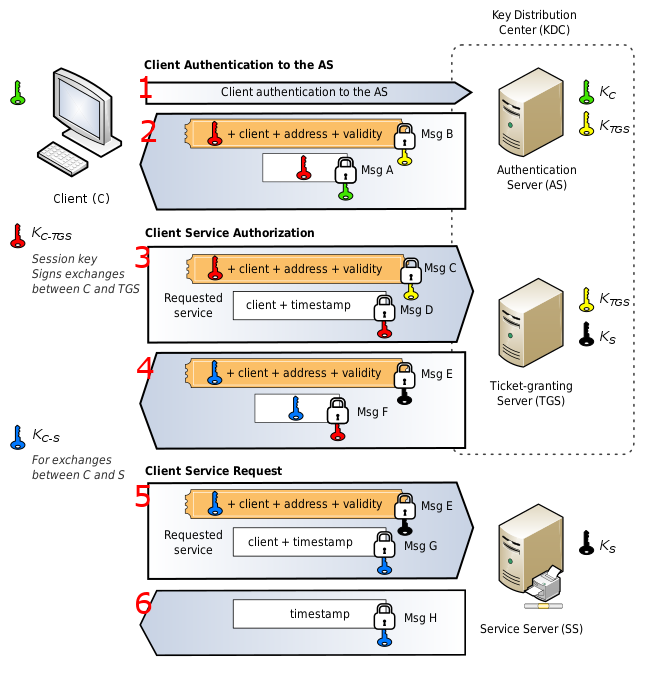
\includegraphics[width=10cm, keepaspectratio]{capitoli/autenticazione/imgs/kerberos1.png}
    \caption{Schema di funzionamento del protocollo Kerberos.}
\end{figure}

\begin{enumerate}
    \item L’utente si connette con le proprie credenziali alla workstation e
          queste vengono passate al Kerberos;
    \item AS verifica il diritto di accesso dell’utente, ricercando una
          corrispondenza nel database. Se il confronto ha esito positivo, AS
          assegna all’user un ticket e una session key.
          Il ticket verrà poi passato al TGS per richiedere i servizi, mentre
          la chiave permette di codificare le sue richieste, sempre poste al TGS.
          Entrambe le informazioni vengono criptate;
    \item L’utente a questo punto vuole utilizzare un certo servizio.
          La workstation richiede all'utente la password e la utilizza per
          decrittografare il messaggio in arrivo, quindi invia ticket e
          autenticatore
          (che contiene il nome, la rete, l'indirizzo e l'ora dell'utente) a TGS;
    \item TGS decripta il ticket e l'autenticatore, verifica se esso ha il
          diritto o meno ad utilizzare una certa risorsa e crea il ticket
          specifico per il servizio richiesto. La comunicazione tra utente e
          TGS avviene solo grazie alla session key che la codifica;
    \item La workstation manda ticket e autenticatore al server;
    \item Il server verifica il match tra ticket ed autenticatore e permette
          l’accesso al servizio. Se
          viene richiesta una mutua autenticazione, il server ritorna un
          autenticatore.
\end{enumerate}

È importante notare che l’utente può utilizzare il ticket finché esso risulta
ancora valido, il che può accadere anche per più tentativi di richiesta al servizio.
Per un servizio diverso mai utilizzato, deve ripercorrere il medesimo processo.\\

Kerberos opera fondamentalmente in \textbf{3 fasi}.

%% TODO: continuare da pagina 31
\chapter{Intruder}

Abbiamo tre classi di intruders (intrusi):

\begin{itemize}
    \item \textbf{Masquerader}: Un individuo che non è autorizzato a utilizzare il
          computer e che penetra nei
          controlli di accesso di un sistema per sfruttare l'account di un utente
          legittimo;
    \item \textbf{Misfeasor}\footnote{Ricordarsi che non è
              il nome di un pokemon !}: Un utente legittimo che accede a dati,
          programmi o
          risorse per i
          quali tale
          accesso non è autorizzato o che è autorizzato a tale accesso ma
          abusa dei suoi
          privilegi;
    \item \textbf{Clandestine User}: Una persona che prende il controllo di supervisione
          per eludere l'auditing
          e i controlli di accesso o sopprimere la raccolta di audit;
\end{itemize}

\paragraph{Intrusion Detection System: }
L'Intrusion Detection System o \textbf{IDS} è un dispositivo software o hardware
utilizzato per
identificare accessi non autorizzati ai computer o alle reti locali.
Le intrusioni rilevate possono
essere quelle prodotte da cracker esperti, da tool automatici o da utenti
inesperti che utilizzano
programmi semiautomatici.

Lo scopo generale di un IDS è informare che potrebbe esserci un'intrusione nella rete. Gli avvisi
includono generalmente informazioni sull'indirizzo di origine dell'intrusione,
l'indirizzo di
destinazione/vittima e il tipo di attacco sospetto”.
Due sono le categorie base: sistemi basati sulle firme (signature) e sistemi
basati sulle anomalie (anomaly).
La tecnica basata sulle firme è in qualche modo analoga a quella per
il rilevamento dei
virus (adopera il machine learning), essa permette di bloccare file infetti e
si tratta di una tra le tecniche più utilizzate. I sistemi basati sul rilevamento delle anomalie utilizzano un
insieme di regole che
permettono di distinguere ciò che è "normale" da ciò che è "anormale".
È importante sapere che un IDS non può bloccare o filtrare i pacchetti in ingresso
ed in uscita, né
tanto meno può modificarli. Un IDS può essere paragonato ad un antifurto mentre
il firewall alla
porta blindata. L'IDS non cerca di bloccare le eventuali intrusioni, cosa che
spetta al firewall, ma
cerca di rilevarle laddove si verifichino.
Per ogni rete è necessario un IDS che agisce solo sulla stessa. Se si volesse
però avere
un'architettura più complessa, si potrebbe includere un gestore centrale:
gli IDS fanno da sensore,
inviano tutto c'è che rilevano nella rete di pertinenza al gestore,
il quale accumula ed analizza tutti i
log ricevuti per capire se gli eventi hanno una qualche correlazione.

\paragraph{Honeypot: } %% TODO: aggiungere emoji
Un honeypot rappresenta una strategica misura di sicurezza con la quale gli
amministratori
di un server ingannano gli hacker e gli impediscono di colpire.
Un “barattolo di miele” simula i
servizi di rete o programmi per attirare i malintenzionati e proteggere il
sistema da eventuali
attacchi. In pratica gli utenti configurano gli honeypot, utilizzando delle
tecnologie lato server e lato
client. Solitamente la trappola consiste in un computer o un sito che sembra
essere parte della rete
e contenere informazioni preziose, ma che in realtà è ben isolato e non ha
contenuti sensibili o
critici; potrebbe anche essere un file, un record, o un indirizzo IP non utilizzato.
Il valore primario di un honeypot è l'informazione che esso dà sulla natura e la
frequenza di
eventuali attacchi subiti dalla rete.
Gli honeypot possono portare dei rischi ad una rete e devono essere maneggiati
con cura. Se non
sono ben protetti, un attacker potrebbe usarli per entrare in altri sistemi.

Gli honeypot possono essere di due tipi:
\begin{itemize}
    \item \textbf{Bassa Interazione}: sono macchine facili da gestire. Emulano perfettamente
          i servizi, ma l'intruder non riesce a prendere completamente il controllo in
          quanto la macchina è vuota;
    \item \textbf{Alta Interazione}: macchine dove vi è effettivamente un servizio e
          l'utente può utilizzarlo.
          Sono la tipologia migliore perché più realistiche ma sono più complesse
          da gestire;
\end{itemize}


%%pagina 28, su NB, frase con falsi positivi sembra sbagliata. dovrebbe essere
%% - falsi positivi basso
%% - falsi negativi alto (forse è meglio questa)
%% ha sbagliato tutti i falsi positivi/negativi

%% KERBEROS
%% A: utente
%% T1: timestamp 1
%% {}k: criptato con chiave K
%% 
%%
%%
%%
%%
%%
%%
%%